\documentclass[12pt]{article}
\usepackage[all, stdclass]{lix}
\usepackage{graphicx}
\usepackage{svg}
\usepackage{circuitikz}
\svgsetup{
  inkscapepath=assets/,  % Path to the directory containing your SVG files
  svgpath=assets/        % Path to the directory containing your SVG files
}
\usepackage{float}
\usepackage{hyperref}
\usepackage{times}
\usepackage{amsmath}
\usepackage{pgfplots}
\usepackage{pdfpages}
\usepackage{subcaption}
\usepackage{caption}
%----------EDIT COVER INFO HERE -----------------%

\def \LOGOPATH {assets/birzeit-logo.png}
\def \DEPARTEMENT {Department of Electrical \& Computer Engineering}
\def \COURSENUM {ENEE2103}
\def \COURSENAME {Circuits and Electronics Laboratory}
\def \REPORTTITLE {Operational Amplifiers}
\def \STUDENTNAME {Mohammad Abu-Shelbaia}
\def \STUDENTID {1200198}
\def \INSTRUCTOR {Dr. Mahran Quraan}
\def \ASSISTANT {Eng. Rafah Rahhal}
\def \PARTNERAN {Nidal Zabade}
\def \PARTNERBN {Mahmoud Shihab}
\def \PARTNERAID {1200153}
\def \PARTNERBID {1182143}
\def \REPORTNUM {10}

\begin{document}
\pagenumbering{Roman}

\begin{titlepage}
    \vfill
    \begin{center}
        \includegraphics[width=0.7\textwidth]{\LOGOPATH} \\
        \hfill \\
        \Large{\DEPARTEMENT} \\
        \Large{\COURSENUM\;-\;\COURSENAME} \\
        \vfill
        \textbf{\LARGE{Experiment \#\REPORTNUM}} \\
        \textbf{\LARGE{\REPORTTITLE}}
    \end{center}
    \vfill
    \begin{flushleft}
        \Large{\textbf{Prepared by:}\\ \STUDENTNAME\quad\STUDENTID} \\
        \Large{\textbf{Partners:}\\
            \begin{tabular}{@{}l@{\quad}l}
                \PARTNERAN & \PARTNERAID \\
                \PARTNERBN & \PARTNERBID \\
            \end{tabular}} \\
        \Large{\textbf{Instructor:} \INSTRUCTOR} \\
        \Large{\textbf{Assistant:} \ASSISTANT} \\
        \Large{\textbf{Section:} 4}\\
        \LARGE{\textbf{ }}\\
        \LARGE{\textbf{ }}\\
        \LARGE{\textbf{ }}\\
        \Large{\textbf{Date:} \today}\\
    \end{flushleft}
    \vfill
\end{titlepage}
{
\centering
\section*{Abstract}
In this experiment, we are going to learn about the different applications of the op-amp: adders, voltage followers, comparators, and comparators with hysteresis, and how to use them to build different circuits. The tools used in this experiment are the oscilloscope, the function generator, the variable DC voltage source, the potentiometer, the uA741 op-amp, and resistors.
}
\clearpage

%--------------- TABLES --------------------------------%
\tableofcontents
\clearpage
\setlength{\parskip}{\baselineskip}%
\listoffigures
\clearpage
\listoftables
\clearpage
\pagenumbering{arabic}
%-------------- CONTENT ---------------------%
\h{Theory}
\hh{Operational Amplifier}


An operational amplifier (op-amp) is a three-terminal device, with two inputs and usually one output, The inputs are labeled as "Inverting Input" and "Non-Inverting Input" and they are marked as "-" and "+" respectively, the inputs have high impedances while the output has low impedance, also the op-amp has a very high gain. The op-amps have three configurations:
\begin{itemize}
    \item Negative Feedback: Usually used in amplifiers and filters.
    \item Positive Feedback: Usually used in oscillators and comparators with hysteresis.
    \item No Feedback (Open Loop): Usually used as a comparator.
\end{itemize}


In the negative feedback configuration, there is a feedback path from the output to the inverting input, and it has many applications such as voltage adders (summer), voltage followers, integrators, differentiators, filters, etc.

In the positive feedback configuration, there is a feedback path from the output to the non-inverting input, and it has some applications such as oscillators and comparators with hysteresis.

In the no feedback configuration, there is no feedback path, and it has some applications such as comparators.

In this experiment, we are going to use the negative feedback configuration to build a voltage follower, an inverting adder, a comparator, and a comparator with hysteresis.
\hh{Inverting Adder}
\begin{figure}[H]
    \centering
    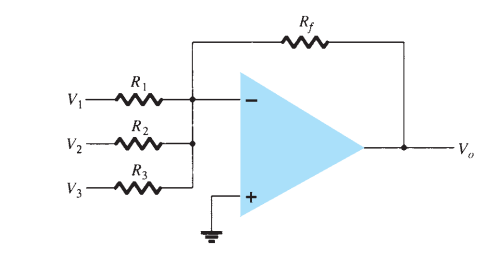
\includegraphics[width=0.7\textwidth]{assets//main/2023-08-27-22-36-03.png}
    \caption{Inverting Adder Amplifier}
    \cite{my_book}
\end{figure}
In the circuit above, assuming that the op-amp is ideal, the current going into the inverting input is zero, and the voltage at the inverting input is equal to the voltage at the non-inverting input, the output voltage is given by:
\begin{equation}
    V_{out} = -(\frac{R_f}{R_{1}}V_1 + \frac{R_f}{R_{2}}V_2 + \frac{R_f}{R_{3}}V_3)
\end{equation}
\hh{Voltage Follower}
\begin{figure}[H]
    \centering
    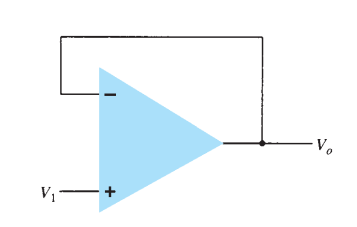
\includegraphics[width=0.5\textwidth]{assets//main/2023-08-27-22-48-49.png}
    \caption{Voltage Follower Amplifier}
    \cite{my_book}
\end{figure}
In the circuit above, assuming that the op-amp is ideal, the current going into the inverting input is zero, and the voltage at the inverting input is equal to the voltage at the non-inverting input, the output voltage is given by:
\begin{equation}
    V_{out} = V_{in}
\end{equation}
However, since the op-amp is not ideal, the output voltage might be slightly less than the input voltage, furthermore, the op-amp has a maximum output current, so if the output current exceeds the maximum output current, the output voltage will saturate.
\hh{Comparator}
\begin{figure}[H]
    \centering
    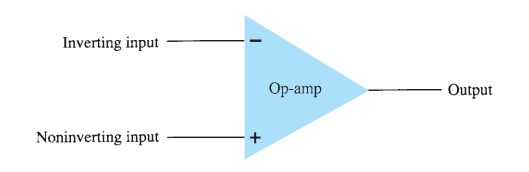
\includegraphics[width=0.7\textwidth]{assets//main/main/2023-08-27-22-55-04.png.png}
    \caption{Comparator Amplifier}
    \cite{my_book}
\end{figure}
In the circuit above, assuming that the op-amp is ideal:
\begin{equation}
    V_{\text{out}} = \begin{cases} 
        -V_{\text{sat}} & \text{if } V_{-} > V_{+} \\
        +V_{\text{sat}} & \text{if } V_{-} < V_{+} \\
    \end{cases}
\end{equation}

\hh{Comparator with Hysteresis (Schmitt Trigger)}
\begin{figure}[H]
    \centering
    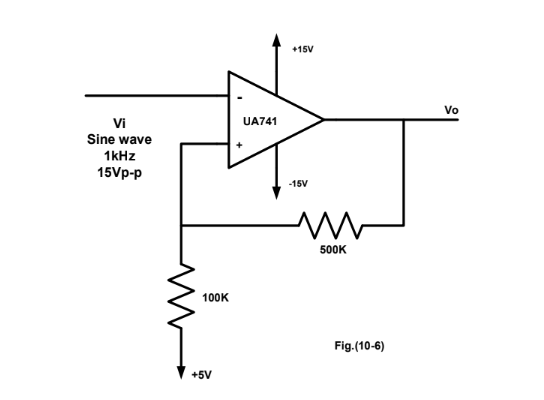
\includegraphics[width=0.6\textwidth]{assets/main/2023-08-27-19-57-16.png}
    \caption{Comparator with Hysteresis Amplifier}
    \cite{manual}
\end{figure}
In the circuit above, assuming that the op-amp is ideal and that the output voltage is either $V_{sat}$ or -$V_{sat}$:
\begin{equation}
    V_{\text{upper}} = \frac{R_1}{R_1 + R_2}V_{\text{sat}} + V_{\text{ref}}
\end{equation}
\begin{equation}
    V_{\text{lower}} = \frac{R_1}{R_1 + R_2}-V_{\text{sat}} + V_{\text{ref}}
\end{equation}
Where:
\begin{itemize}
    \item $V_{\text{upper}}$ is the upper trigger level.
    \item $V_{\text{lower}}$ is the lower trigger level.
    \item $V_{\text{sat}}$ is the saturation voltage of the op-amp.
    \item $V_{\text{ref}}$ is the reference voltage (Voltage on the resistor assuming $V_{out}$ is connected to the ground).
    \item $R_1 = 100k\Omega$ and $R_2 = 600k\Omega$ are the resistors in the voltage divider.
\end{itemize}

\clearpage
\h{Procedure and Data Analysis}
\hh{Adding Application}
\begin{figure}[H]
    \centering
    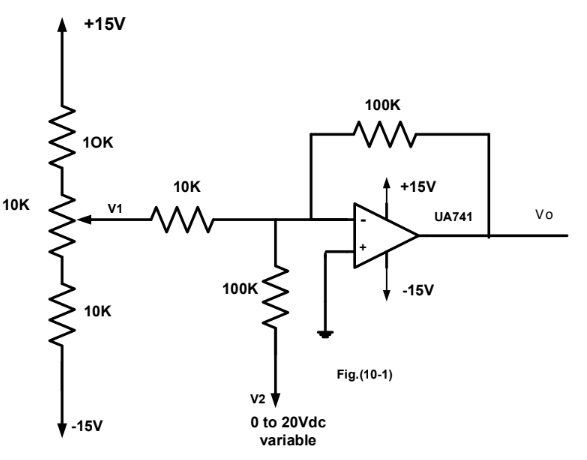
\includegraphics[width=0.7\textwidth]{assets/main/2023-08-27-18-37-15.png}
    \caption{Inverting Adder Amplifier}
    \cite{manual}
    \label{fig:1}
\end{figure}
The circuit above was connected to a variable DC voltage source and the output was measured. Since this is an inverting amplifier, the output voltage is given by:
\begin{equation}
    V_{out} = -(\frac{R_f}{R_{1}}V_1 + \frac{R_f}{R_{2}}V_2) = -(\frac{100k}{10k}V_1 + \frac{100k}{100k}V_2) = -10V_1 - V_2
    \label{eq:1}
\end{equation}
The output voltage was measured for different values of $V_1$ and $V_2$ and the results are shown in (Table \ref{tab:1}).

\begin{table}[H]
    \centering
    \resizebox{0.5\textwidth}{!}{%
        \begin{tabular}{|cc|cc|}
            \hline
            \multicolumn{2}{|c|}{Input Voltage} & \multicolumn{2}{c|}{Output Voltage}                                                   \\ \hline
            \multicolumn{1}{|c|}{$V_{in1}$}     & $V_{in2}$                           & \multicolumn{1}{c|}{$V_o$} & Calculated Voltage \\ \hline
            \multicolumn{1}{|c|}{0.5}           & 2                                   & \multicolumn{1}{c|}{-7.05} & -7                 \\ \hline
            \multicolumn{1}{|c|}{0.3}           & 4                                   & \multicolumn{1}{c|}{-6.95} & -7                 \\ \hline
            \multicolumn{1}{|c|}{-0.9}          & 2                                   & \multicolumn{1}{c|}{6.88}  & 7                  \\ \hline
            \multicolumn{1}{|c|}{-1.5}          & 6                                   & \multicolumn{1}{c|}{8.92}  & 9                  \\ \hline
        \end{tabular}%
    }
    \caption{Inverting Adder Amplifier Voltages}
    \label{tab:1}
\end{table}
The Calculated Voltage column was calculated using (Equation \ref{eq:1}). The results show that the output voltage matches the calculated voltage with a small error. This error is because the resistors used in the circuit are not ideal and have a small tolerance and the fact that the op-amp is not ideal either.
\hh{Voltage Follower Application}
\begin{figure}[H]
    \centering
    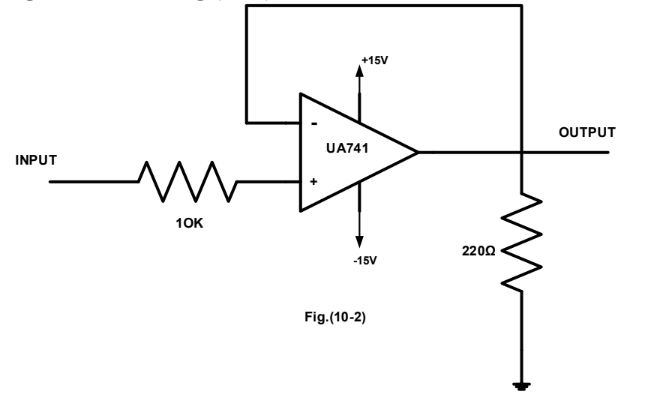
\includegraphics[width=0.7\textwidth]{assets//main/2023-08-27-18-59-49.png}
    \caption{Voltage Follower Amplifier}
    \label{fig:2}
    \cite{manual}
\end{figure}
The circuit above was connected to a variable DC voltage source and the output was measured. Since this is a voltage follower, the output voltage is given by:
\begin{equation}
    V_{out} = V_{in}
    \label{eq:2}
\end{equation}
The output voltage was measured for different values of $V_{in}$ and two different values of $R_f$ and the results are shown in (Table \ref{tab:2}).
% Please add the following required packages to your document preamble:
% \usepackage{graphicx}
\begin{table}[H]
    \resizebox{\textwidth}{!}{%
        \begin{tabular}{|l|l|l|l|l|l|l|l|l|l|l|l|}
            \hline
            \multicolumn{1}{|c|}{$V_{in}$} & 1    & 3    & 4    & 5    & 6    & 7    & 8    & 10    & 12    & 14   & 15   \\ \hline
            $V_o [220\Omega]$              & 1.01 & 3.02 & 4.06 & 5.04 & 5.73 & 5.75 & 5.75 & 5.76  & 5.76  & 5.73 & 6.73 \\ \hline
            $V_o [1k\Omega]$               & 1.06 & 3.12 & 4.15 & 5.17 & 6.2  & 7.2  & 8.07 & 10.03 & 12.09 & 12.9 & 12.9 \\ \hline
        \end{tabular}%
    }
    \caption{Voltage Follower Amplifier Voltages}
    \label{tab:2}
\end{table}
We can see that initially, the output voltage matches the input voltage, but as the input voltage increases, the output voltage starts to saturate at around 5.75V for the 220$\Omega$ resistor and 12.9V for the 1k$\Omega$ resistor. This is due to the maximum output current of the op-amp being limited the maximum current that we could get from the op-amp is
\begin{equation}
    5.75V/220\Omega = 26mA\quad and \quad 12.9V/1k\Omega = 12.9mA
\end{equation} The circuit has a similar behavior to an emitter follower circuit with a BJT transistor.
\hh{Comparator Application}
\begin{figure}[H]
    \centering
    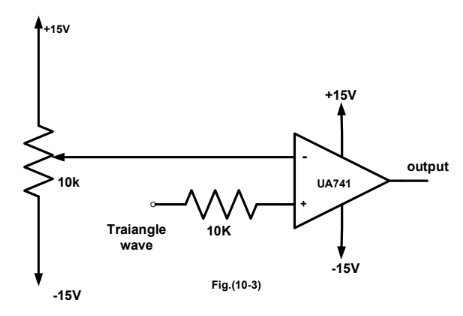
\includegraphics[width=0.7\textwidth]{assets/main/2023-08-27-19-19-20.png}
    \caption{Comparator Amplifier}
    \label{fig:3}
    \cite{manual}
\end{figure}
The circuit above was connected to a function generator and it was set to generate a triangle wave with a frequency of 1kHz and a peak-to-peak voltage of 2V. The potentiometer was used as a voltage divider to change the reference voltage.
\begin{figure}[H]
    \begin{subfigure}[b]{0.49\textwidth}
        \centering
        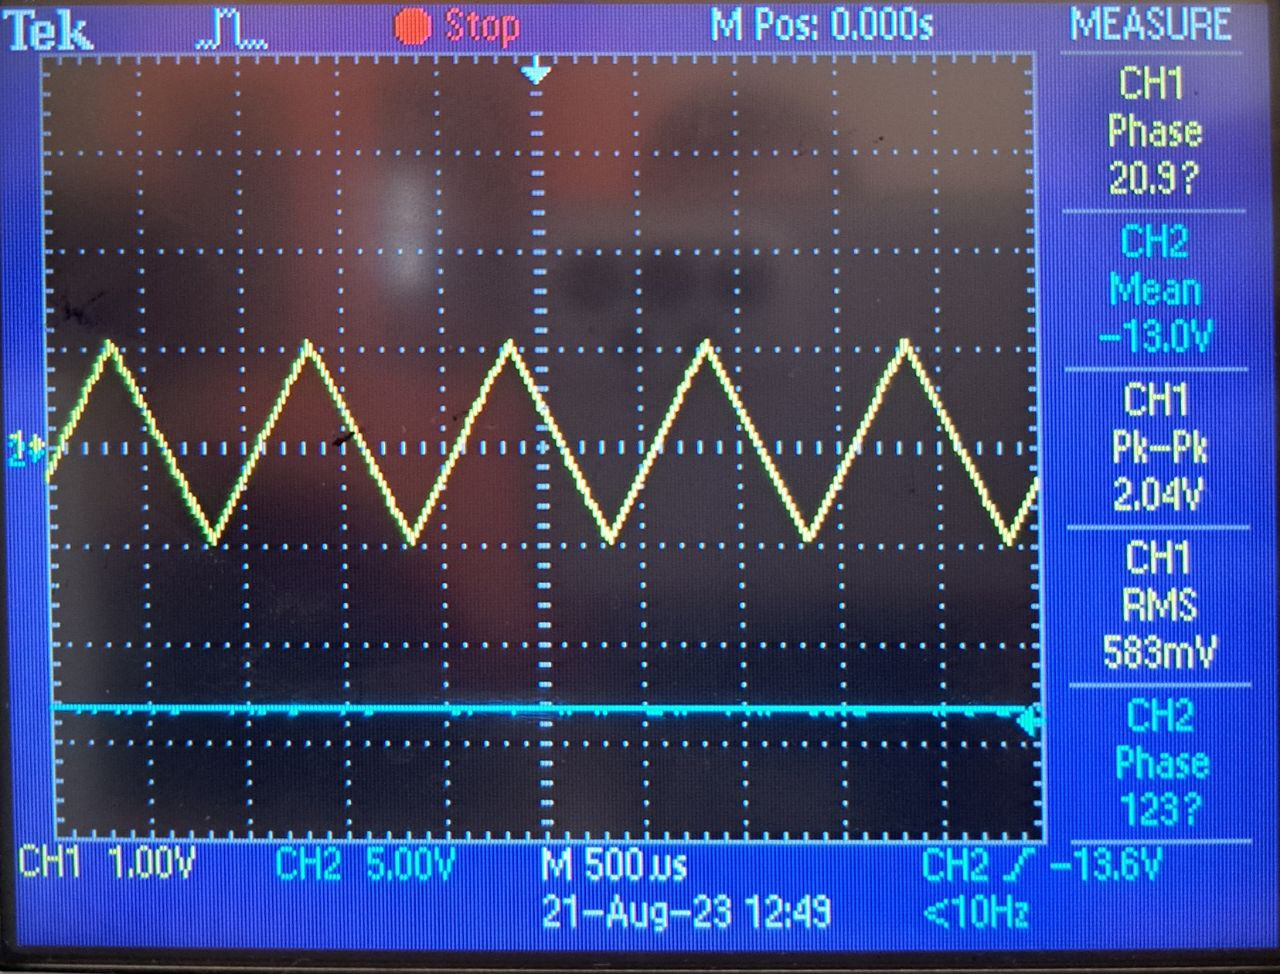
\includegraphics[width=\textwidth]{assets//main/2023-08-27-19-32-52.png}
        \subcaption{$V_{-} > V_{+}$}
    \end{subfigure}
    \begin{subfigure}[b]{0.49\textwidth}
        \centering
        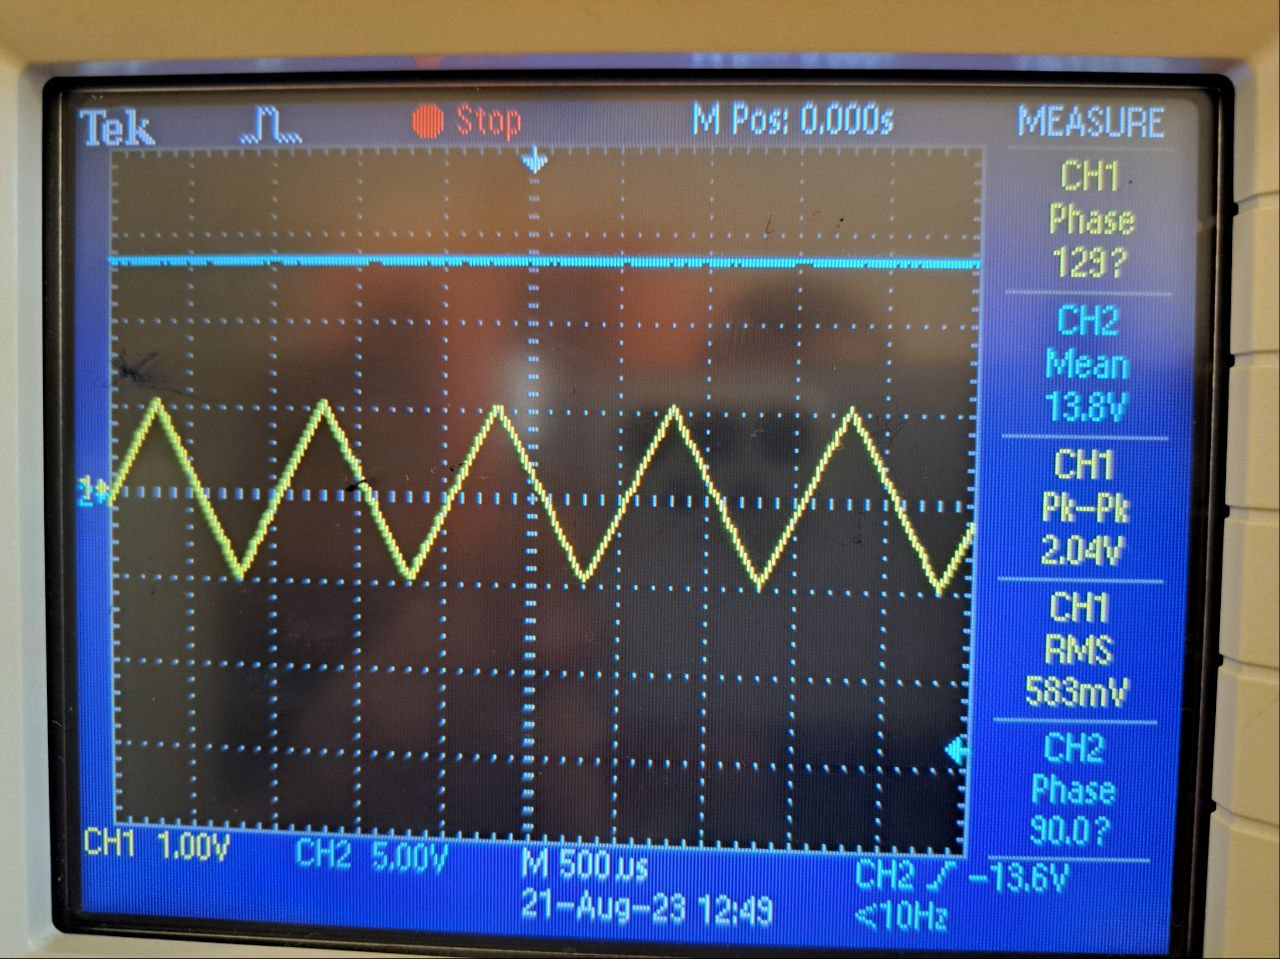
\includegraphics[width=\textwidth]{assets//main/2023-08-27-19-37-42.png}
        \subcaption{$V_{-} < V_{+}$}
    \end{subfigure}
    \caption{Comparator Amplifier Output}
\end{figure}
We observed that when $V_{-} > V_{+}$, the output voltage is -$V_{sat}$ and when $V_{-} < V_{+}$, the output voltage is $V_{sat}$ Where $V_{sat}$ is the saturation voltage of the op-amp and it is around 15V, $V_{-}$ is the AC voltage and $V_{+}$ is the reference DC voltage.
\\
Furthermore, we changed the DC reference voltage to around 0V and we observed that we get a square wave with a positive amplitude when $V_{-} > V_{+}$ and a negative amplitude when $V_{-} < V_{+}$.
\begin{figure}[H]
    \centering
    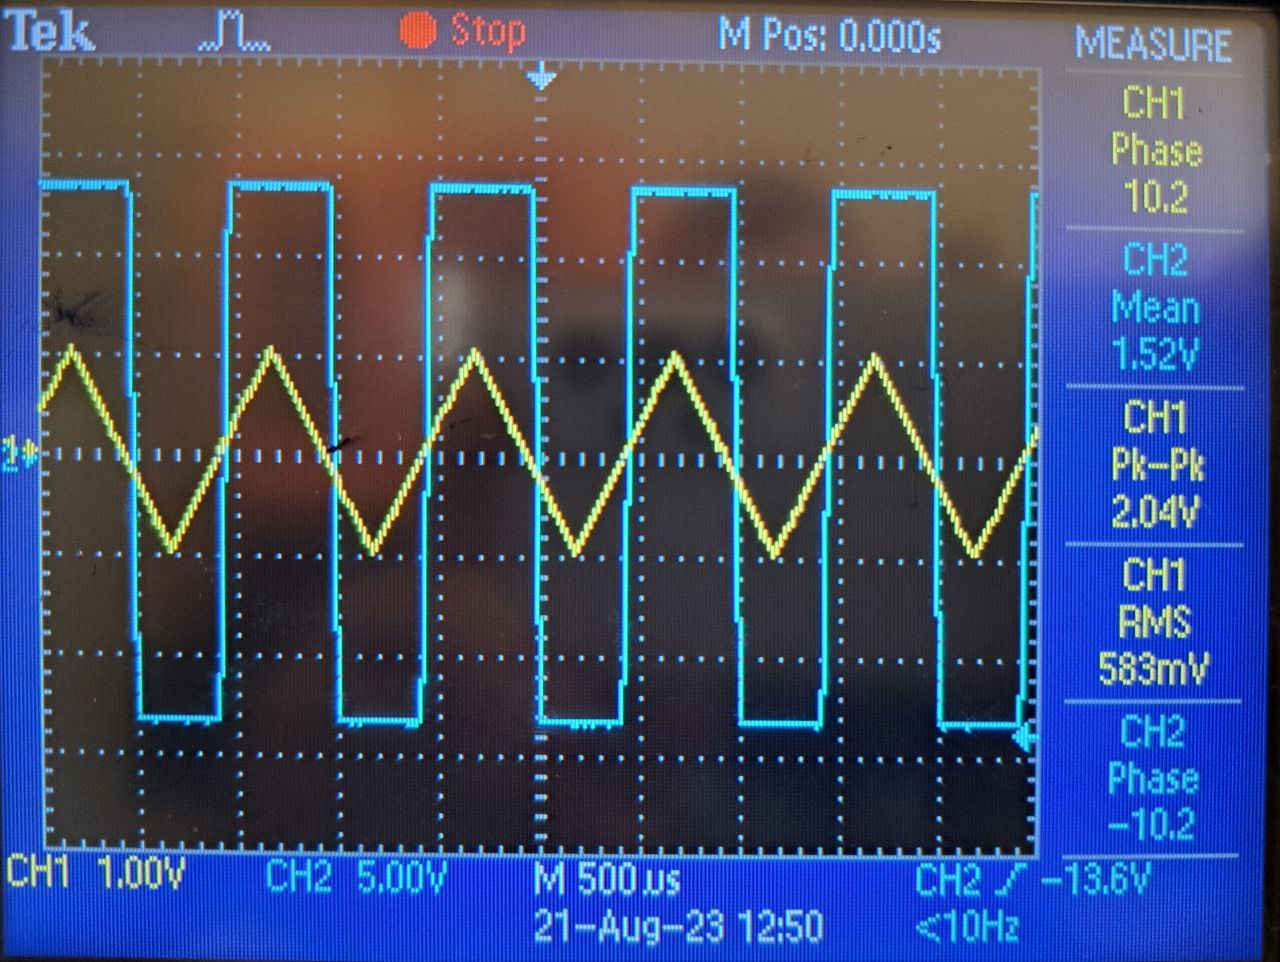
\includegraphics[width=0.425\textwidth]{assets//main/2023-08-27-19-45-30.png}
    \caption{Comparator Amplifier Output [Square Wave]}
    \label{fig:4}
\end{figure}
\hh{Comparator with Hysteresis Application}
\begin{figure}[H]
    \centering
    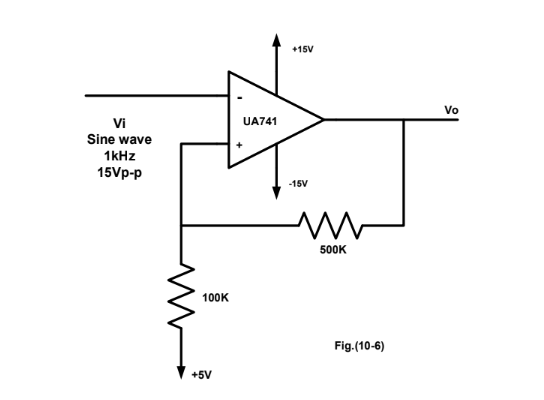
\includegraphics[width=0.7\textwidth]{assets/main/2023-08-27-19-57-16.png}
    \caption{Comparator with Hysteresis Amplifier}
    \label{fig:5}
    \cite{manual}
\end{figure}
The circuit above was connected to a function generator and it was set to generate a sine wave with a frequency of 1kHz and a peak-to-peak voltage of 15V. The output signal was plotted and it is shown in (Figure \ref{fig:6}).
\begin{figure}[H]
    \centering
    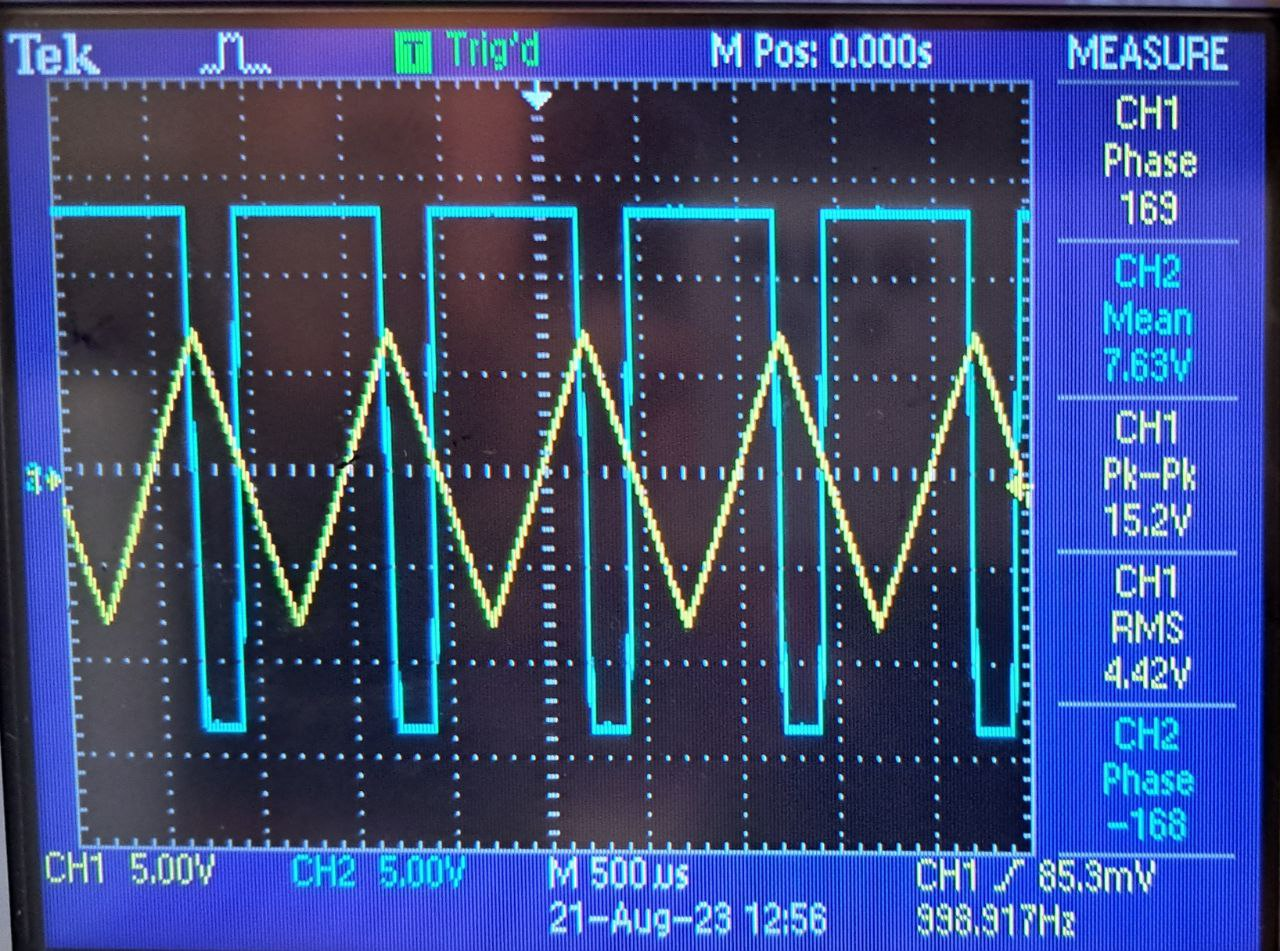
\includegraphics[width=0.425\textwidth]{assets//main/2023-08-27-20-01-04.png}
    \caption{Comparator with Hysteresis Amplifier Output}
    \label{fig:6}
\end{figure}

\begin{figure}[H]
    \begin{subfigure}[b]{0.49\textwidth}
        \centering
        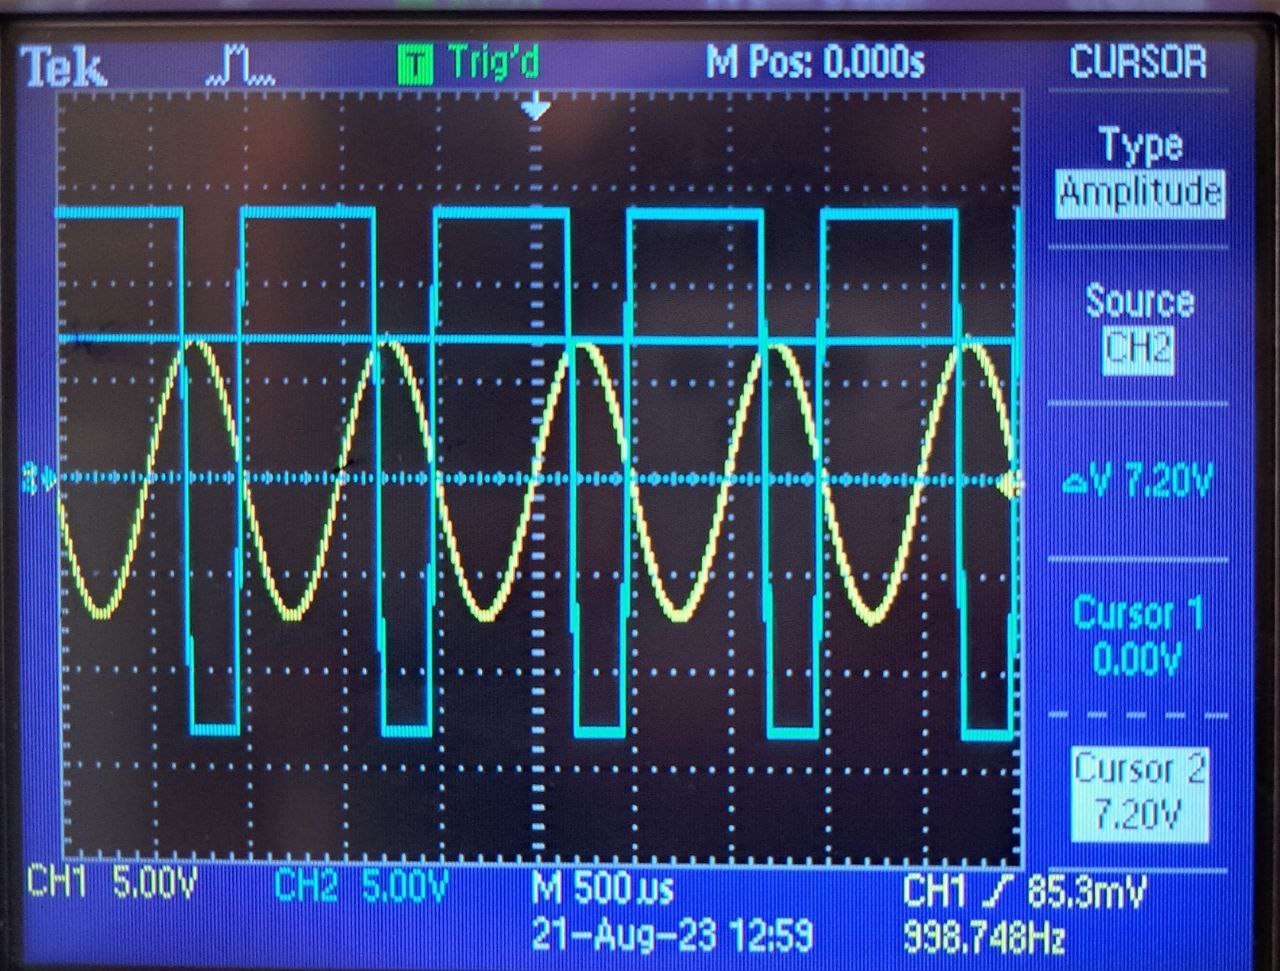
\includegraphics[width=\textwidth]{assets//main/2023-08-27-20-03-47.png}
        \subcaption{Upper Trigger Level}
    \end{subfigure}
    \begin{subfigure}[b]{0.49\textwidth}
        \centering
        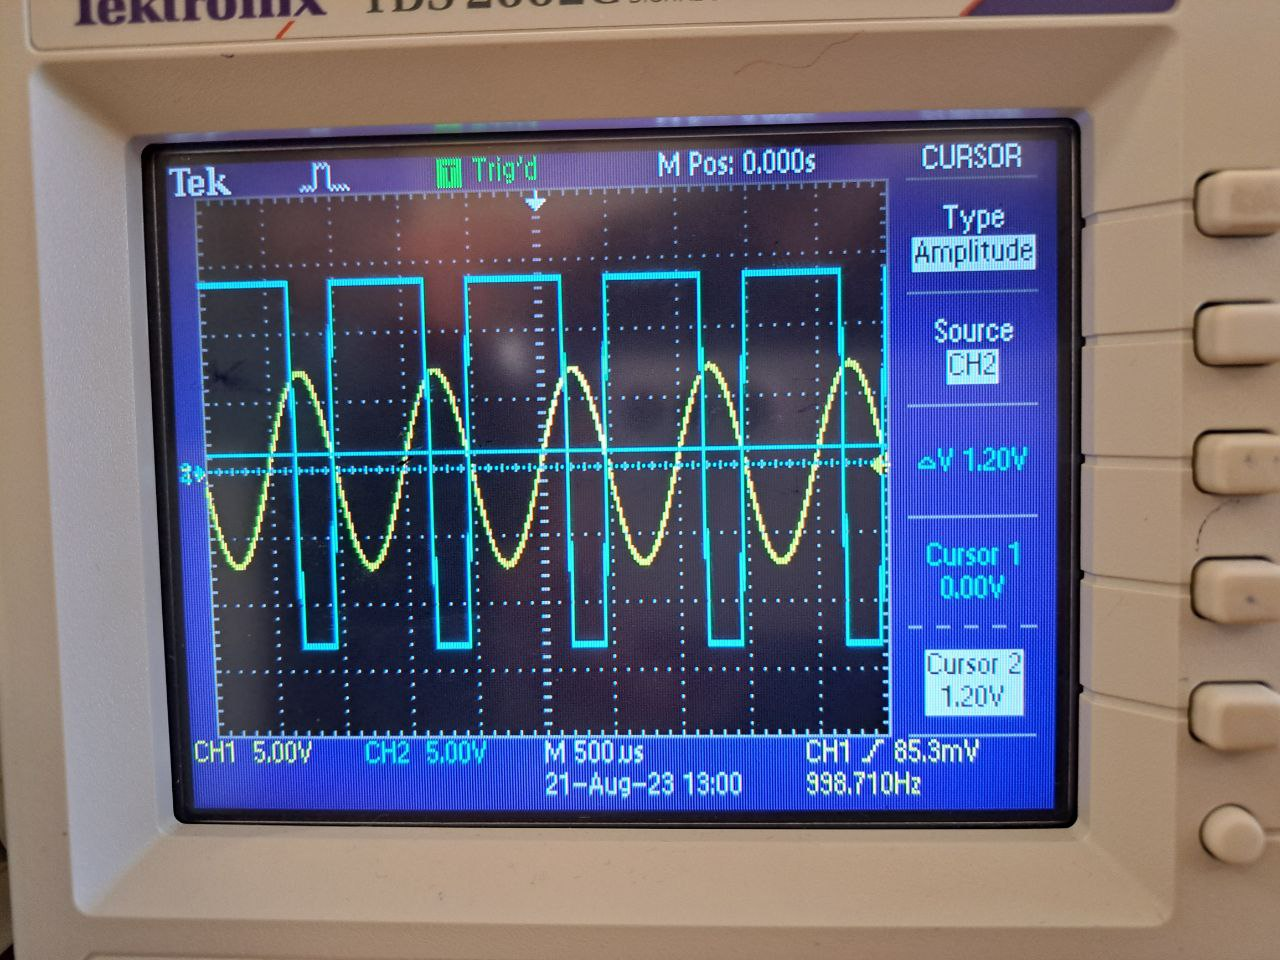
\includegraphics[width=\textwidth]{assets//main/2023-08-27-20-04-03.png}
        \subcaption{Lower Trigger Level}
    \end{subfigure}
    \caption{Comparator Trigger Levels}
\end{figure}
From the oscilloscope, we measured the upper trigger level to be around 7.2V and the lower trigger level to be around 1.2V. The theoretical values for the upper and lower trigger levels using super-position are:
\begin{equation}
    V_{upper} = {100K \over 100k + 500k}\times V_{sat} + 5 \times {500K \over 100k + 500k}= 6.667V
\end{equation}
\begin{equation}
    V_{upper} = {100K \over 100k + 500k}\times -V_{sat} + 5 \times {500K \over 100k + 500k}= 1.667V
\end{equation}

The measured values are close to the theoretical values, but they are not the same. This is because the resistors used in the circuit are not ideal and have a small tolerance and the fact that the op-amp is not ideal either.

\clearpage
\h{Conclusion}
In conclusion, we learned about the different applications of the op-amp and how to use it to build different circuits, the difference between the normal comparator and the comparator with hysteresis, and we discovered that the op-amp is not ideal and has a small error and that the op-amp has some limitations such as the maximum output current.
\clearpage
\bibliographystyle{IEEEtran}
\bibliography{cites}
\clearpage
\h*{Appendix}
\begin{figure}[H]
    \centering
    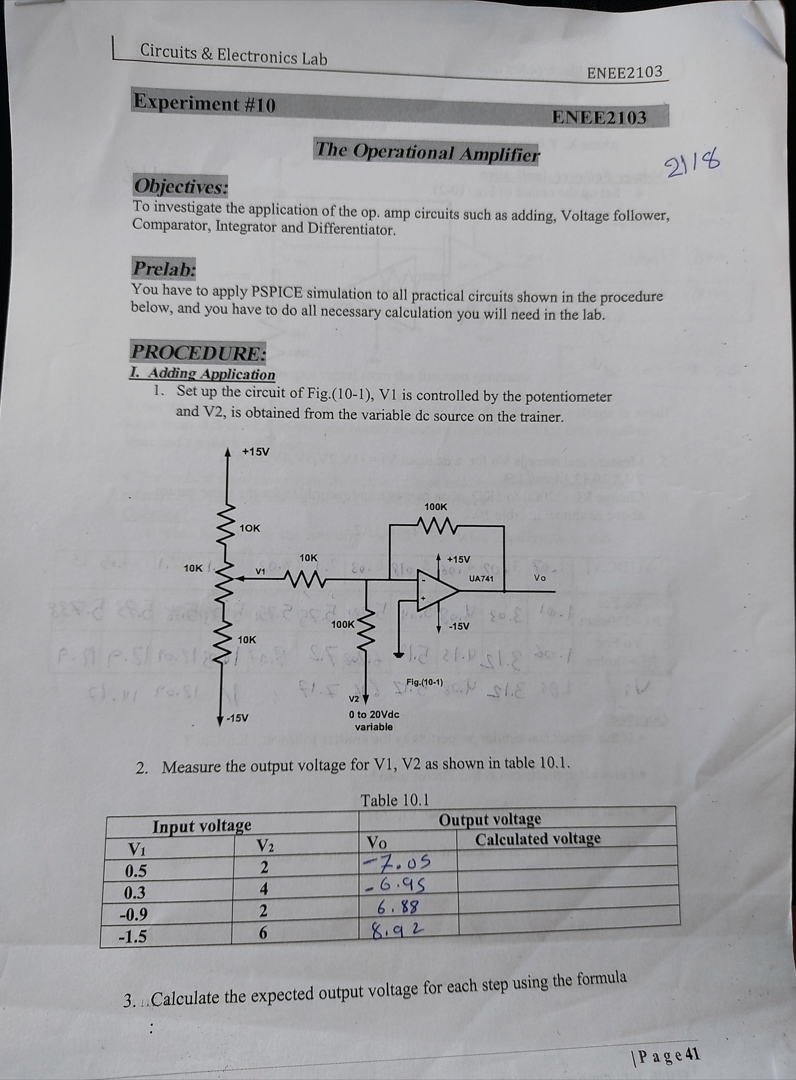
\includegraphics[width=0.8\textwidth]{assets//main/2023-08-27-23-44-18.png}
\end{figure}
\clearpage
\begin{figure}[H]
    \centering
    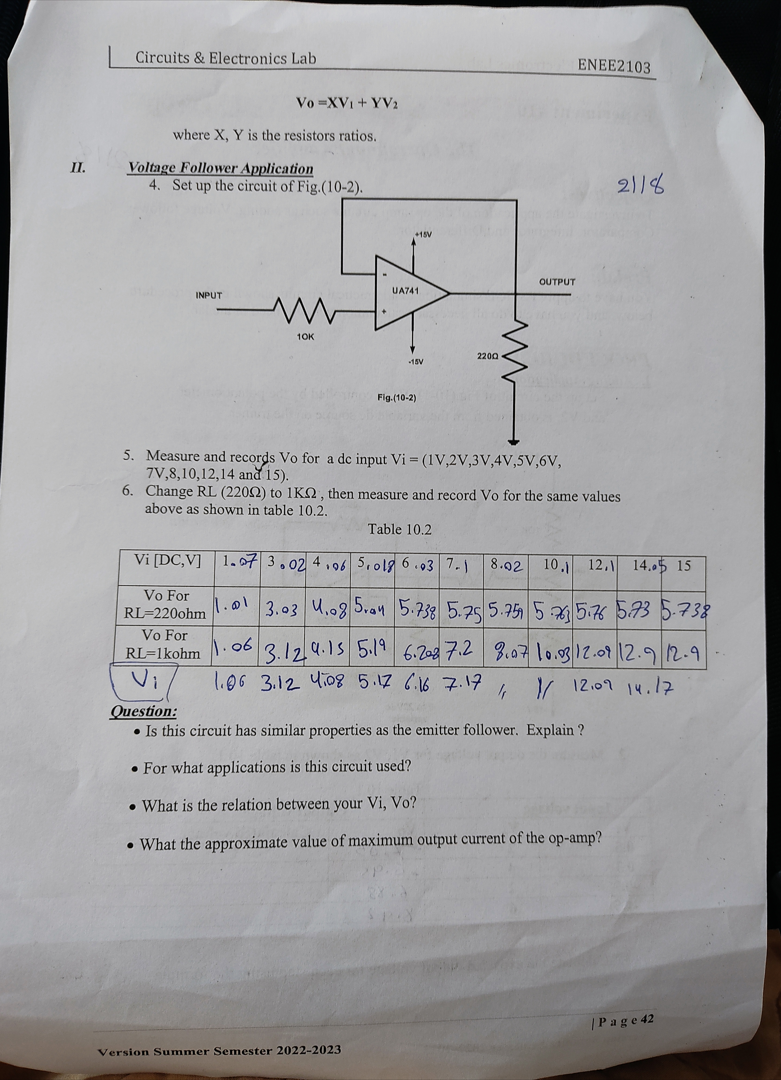
\includegraphics[width=0.8\textwidth]{assets//main/2023-08-27-23-45-46.png}

\end{figure}
\clearpage
\begin{figure}[H]
    \centering  
    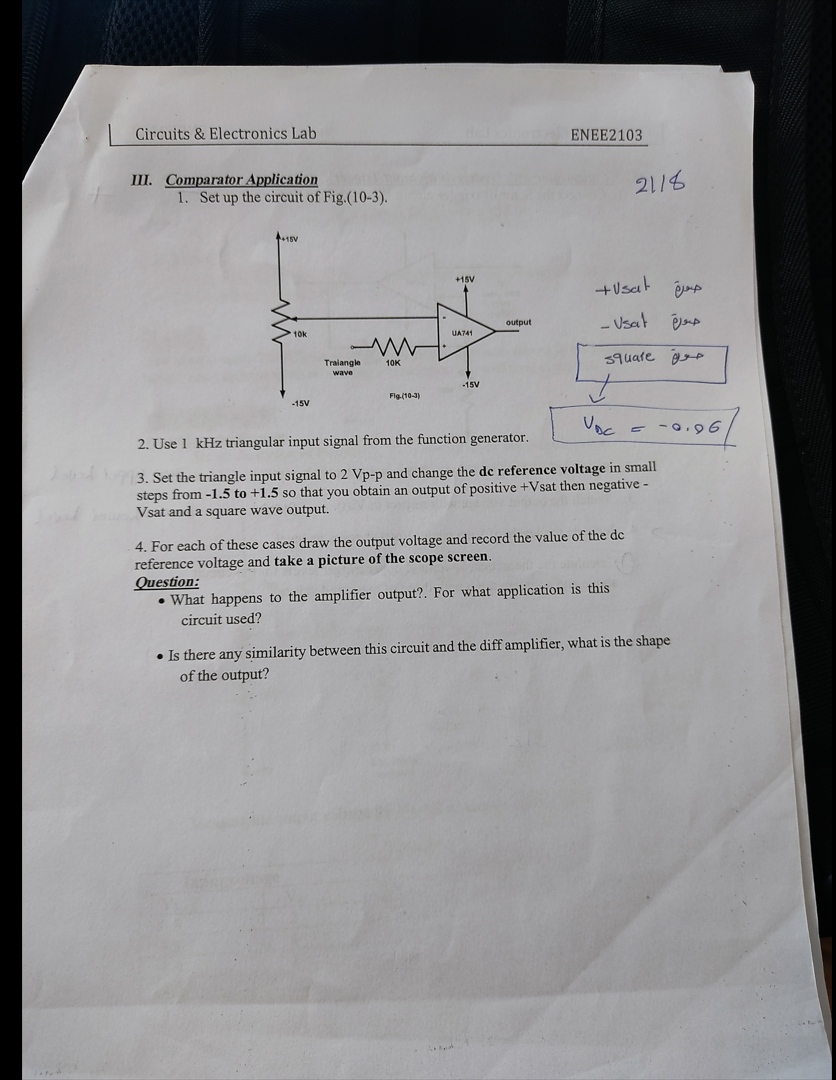
\includegraphics[width=0.8\textwidth]{assets//main/2023-08-27-23-44-51.png}
\end{figure}
\clearpage
\begin{figure}[H]
    \centering
    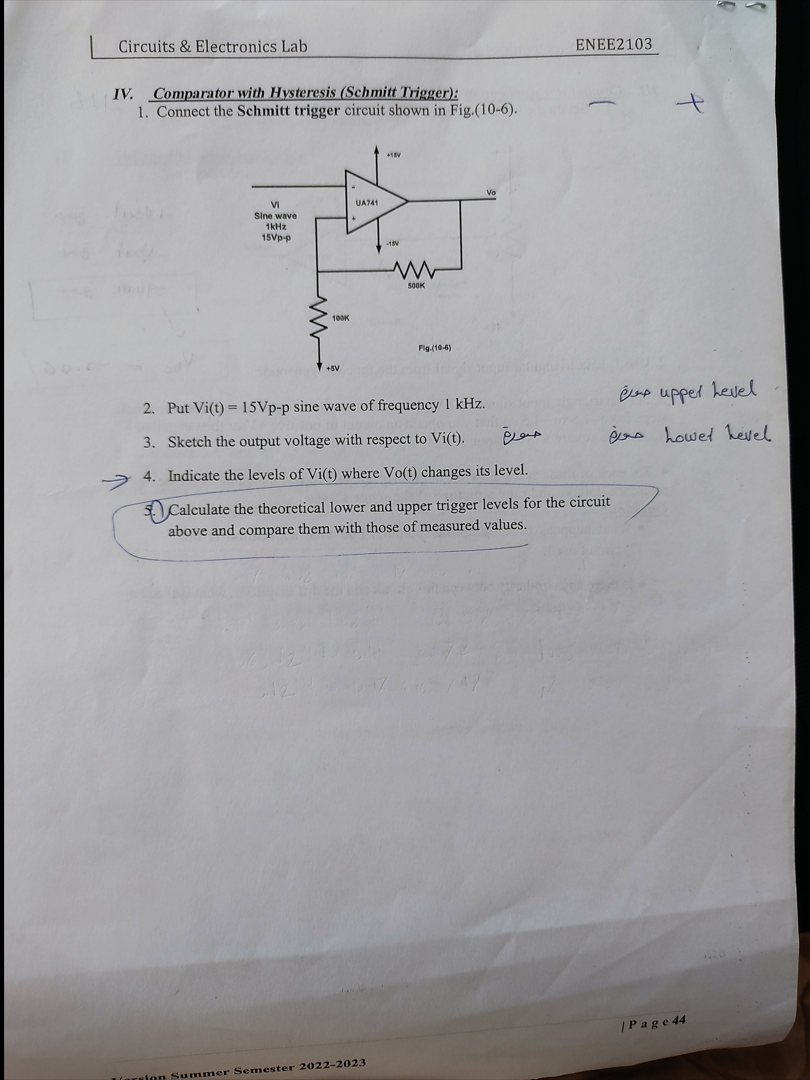
\includegraphics[width=0.8\textwidth]{assets//main/2023-08-27-23-46-18.png}
\end{figure}
\clearpage
\end{document}





